\begin{figure}[b]
  \centering
      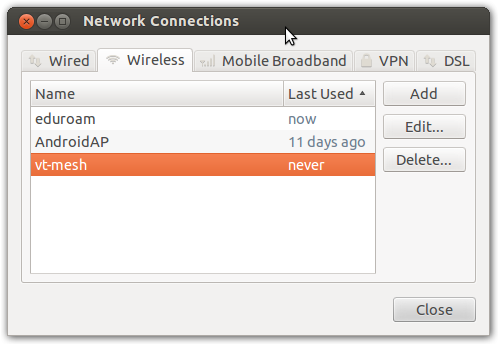
\includegraphics[width=0.7\textwidth]{networkconnections.PNG}
  \caption [Network Connections on Linux Ubuntu]{\textbf{This figure shows the "vt-mesh" under Wireless Network Connections.}}
  \label{fig:networkconnections}
\end{figure}

\begin{figure}[b]
  \centering
      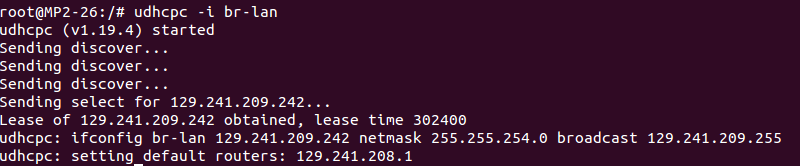
\includegraphics[width=1\textwidth]{sendingdiscover.PNG}
  \caption [The results from executing "uchcpc -i br-lan".]{\textbf{This figure shows the allocation of lease after executing "uchcpc -i br-lan".}}
  \label{fig:sendingdiscover}
\end{figure}

\begin{figure}
        \centering
        \begin{subfigure}[t]{0.49\textwidth}
                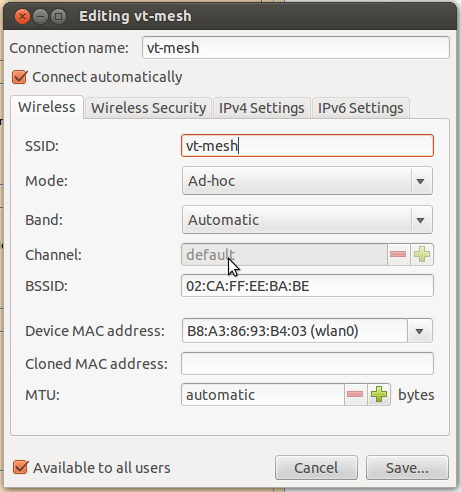
\includegraphics[width=\textwidth]{bssid.PNG}
                \caption{\textbf{The correct BSSID set.}}\label{fig:bssid}
        \end{subfigure}
        \begin{subfigure}[t]{0.49\textwidth}
                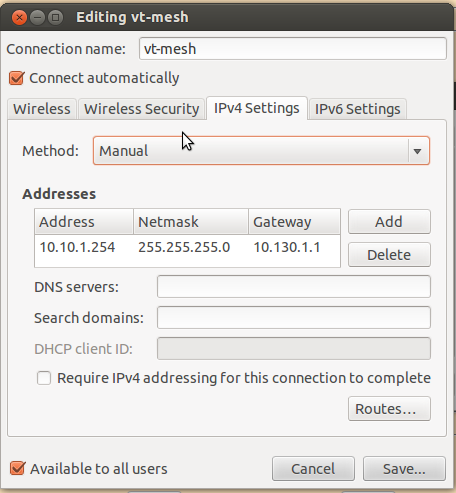
\includegraphics[width=\textwidth]{ipv4settings.PNG}
                \caption{\textbf{The correct parameters set under IPv4 settings.}}\label{fig:ipv4settings}
        \end{subfigure}
\caption{"Edit Connections" settings on Linux}
\end{figure}

One way to get Internet is by connecting the \gls{mp} with an Ethernet cable to the jack port in the wall. This way of receiving internet requires no specific configuration. 

The Mesh Potato is delivered preconfigured with IP address and name of the network (SSID) stated in the \gls{quick} box.


\begin{enumerate}
\item Make sure that you are connected to the \gls{mp} via WiFi on your PC. In order to do this perform the following steps:
\begin{enumerate}
\item Press the WiFi symbol in the top right corner on your Linux Ubuntu home screen, and press "Edit Connections".
\item  Under the tab "Wireless" choose the network called "vt-mesh" and press "Edit" like shown in \fref{fig:networkconnections}.
\item In the field BSSID enter "02:CA:FF:EE:BA:BE", like shown in \fref{fig:bssid}.
\item Under the tab "IPv4 Settings" choose "Manual" under the Method drop-down menu, like shown in \fref{fig:ipv4settings}. 
\item Then press "Add" on the same page. Enter the following parameters, like shown in \fref{fig:ipv4settings}:
\begin{description}
\item[] \textbf{Address:} 10.10.1.245
\item[] \textbf{Netmask:} 24
\item[] \textbf{Gateway:} 10.130.1.1
\end{description}
\item Press "Save" and close the window. 
\item Then choose "vt-mesh" from the list of networks available. The PC should then be connected to the MP via WiFi. 
\end{enumerate}
\item Connect the MP (the LAN-port) to wired Internet (wall jack) with an Ethernet cable.
\item Telnet into the \gls{mp}:
\noindent
\begin{lstlisting}[language=bash]
  $ sudo su
  $ telnet 10.10.1.20
\end{lstlisting}
\item Inside the MP, execute the following command:
\noindent
\begin{lstlisting}[language=bash]
 $ udhcpc -i br-lan
\end{lstlisting}
\item A "Sending discover ..." appears, and a lease is obtained like shown in \fref{fig:sendingdiscover}. 
\end{enumerate}

